\subsection{CU5 Modificar Registro de Vehículo}
Esta pantalla es muy similar a la del 'Registro de Vehículo' (figura \ref{fig:Pantalla Registrar Vehículo - Vista de Escenarios}), solo que esta vez cuando el usuario desee modificar un registro en específico este formulario aparecerá con todos los campos llenos para que el usuario pueda modificar el que necesite. 
\\
En la parte inferior de la pantalla hay dos botones; el primero de ellos, el botón 'Modificar' lleva la información a la base de datos. El segundo, botón 'Cancelar' cierra esta pantalla y no hay alteración en los datos. 
\begin{figure}[!h]
	\centering
	\includegraphics[width=1\textwidth]{./diseno/vescenarios/imagenes/modificarVehículo}
	\caption{Pantalla Modificar Registro de Vehículo - Vista de Escenarios}
	\label{fig:Pantalla Modificar Registro de Vehículo - Vista de Escenarios}
\end{figure}
\\
En caso de que el usuario actualice algún dato mal, es decir, que los campos no estén llenos o el formato de la información no es el correcto, aparecerá una alerta como la que se muestra a continuación (figura \ref{fig:Alerta3 - Vista de Escenarios}):
\begin{figure}[!h]
	\centering
	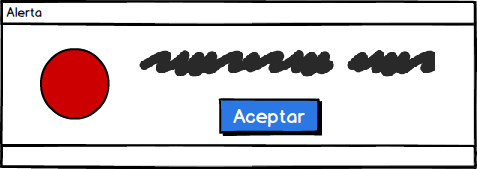
\includegraphics[width=0.5\textwidth]{./diseno/vescenarios/imagenes/alerta}
	\caption{Alerta Modificación - Vista de Escenarios}
	\label{fig:Alerta3 - Vista de Escenarios}
\end{figure}
\clearpage